\documentclass[12pt]{report}
\usepackage[utf8]{inputenc}
\usepackage[russian]{babel}
%\usepackage[14pt]{extsizes}
\usepackage{listings}

% Для листинга кода:
\lstset{ %
language=python,                 % выбор языка для подсветки 
basicstyle=\small\sffamily, % размер и начертание шрифта для подсветки кода
numbers=left,               % где поставить нумерацию строк (слева\справа)
numberstyle=\tiny,           % размер шрифта для номеров строк
stepnumber=1,                   % размер шага между двумя номерами строк
numbersep=5pt,                % как далеко отстоят номера строк от подсвечиваемого кода
showspaces=false,            % показывать или нет пробелы специальными отступами
showstringspaces=false,      % показывать или нет пробелы в строках
showtabs=false,             % показывать или нет табуляцию в строках            
tabsize=2,                 % размер табуляции по умолчанию равен 2 пробелам
captionpos=t,              % позиция заголовка вверху [t] или внизу [b] 
breaklines=true,           % автоматически переносить строки (да\нет)
breakatwhitespace=false, % переносить строки только если есть пробел
escapeinside={\#*}{*)}   % если нужно добавить комментарии в коде
}

% Для измененных титулов глав:
\usepackage{titlesec, blindtext, color} % подключаем нужные пакеты
\definecolor{gray75}{gray}{0.75} % определяем цвет
\newcommand{\hsp}{\hspace{20pt}} % длина линии в 20pt
% titleformat определяет стиль
\titleformat{\chapter}[hang]{\Huge\bfseries}{\thechapter\hsp\textcolor{gray75}{|}\hsp}{0pt}{\Huge\bfseries}

\usepackage{amsmath}
\usepackage{mathptmx}
% plot
\usepackage{pgfplots}
\usepackage{filecontents}
\usepackage{amsmath}
\usepackage{tikz,pgfplots}
\usetikzlibrary{datavisualization}
\usetikzlibrary{datavisualization.formats.functions}

\usepackage{geometry}
\geometry{verbose, a4paper,tmargin=2cm, bmargin=2cm, rmargin=1.5cm, lmargin = 3cm}

\usepackage{graphicx}
\graphicspath{{src/}}
\DeclareGraphicsExtensions{.pdf,.png,.jpg}

\begin{document}
%\def\chaptername{} % убирает "Глава"
\begin{titlepage}
	\centering
	{\scshape\LARGE МГТУ им. Баумана \par}
	\vspace{3cm}
	{\scshape\Large Рубежный контроль №2\par}
	\vspace{0.5cm}	
	{\scshape\Large По курсу: "Анализ алгоритмов"\par}
	\vspace{1.5cm}
	{\huge\bfseries Регулярные выражения \par}
	\vspace{2cm}
	\Large Работу выполнила: Маковская Яна, ИУ7-54\par
	\vspace{0.5cm}
	\Large Преподаватели:  Волкова Л.Л., Строганов Ю.В.\par

	\vfill
	\large \textit {Москва, 2019} \par
\end{titlepage}

\tableofcontents

\newpage
\chapter*{Введение}
\addcontentsline{toc}{chapter}{Введение}

Цель работы: изучение возможностей регулярных выражений. Реализация поиска подстроки в файле при использовании регулярных выражений и конечного автомата.
В ходе рубежного контроля предстоит:
\begin{itemize}
	\item Изучить регулярные выражения; 
	\item реализовать алгоритмы поиска ФИО в тексте
\end{itemize}

\chapter{Аналитическая часть}
Регулярные выражения (англ. regular expressions) — формальный язык поиска и осуществления манипуляций с подстроками в тексте, основанный на использовании метасимволов (символов-джокеров, англ. wildcard characters). Для поиска используется строка-образец (англ. pattern, по-русски её часто называют «шаблоном», «маской»), состоящая из символов и метасимволов и задающая правило поиска. Для манипуляций с текстом дополнительно задаётся строка замены, которая также может содержать в себе специальные символы.


\section{Использование регулярных выражений}
Регулярные выражения используются некоторыми текстовыми редакторами и утилитами для поиска и подстановки текста. Например, при помощи регулярных выражений можно задать шаблоны, позволяющие:
\begin{itemize}
	\item найти все последовательности символов «кот» в любом контексте, как то: «кот», «котлета», «терракотовый»;
	\item найти отдельно стоящее слово «кот» и заменить его на «кошка»;
	\item найти слово «кот», которому предшествует слово «персидский» или «чеширский»;
	\item убрать из текста все предложения, в которых упоминается слово кот или кошка.
\end{itemize}
Регулярные выражения позволяют задавать и гораздо более сложные шаблоны поиска или замены.

Результатом работы с регулярным выражением может быть:
\begin{itemize}
	\item проверка наличия искомого образца в заданном тексте;
	\item определение подстроки текста, которая сопоставляется образцу;
	\item определение групп символов, соответствующих отдельным частям образца.
\end{itemize}
Если регулярное выражение используется для замены текста, то результатом работы будет новая текстовая строка, представляющая из себя исходный текст, из которого удалены найденные подстроки (сопоставленные образцу), а вместо них подставлены строки замены (возможно, модифицированные запомненными при разборе группами символов из исходного текста). Частным случаем модификации текста является удаление всех вхождений найденного образца — для чего строка замены указывается пустой.
\section{Регулярные выражения в теории формальных языков}
Регулярные выражения состоят из констант и операторов, которые определяют множества строк и множества операций на них соответственно. Определены следующие константы:
\begin{itemize}
\item (пустое множество) $\emptyset$.
\item (пустая строка) $\epsilon$ обозначает строку, не содержащую ни одного символа; эквивалентно \"".
\item (символьный литерал) "a", где a — символ используемого алфавита.
\item (множество) из символов, либо из других множеств.
и следующие операции:
\end{itemize}
\begin{itemize}
	\item (сцепление, конкатенация) RS обозначает множество ${\alpha\beta | \alpha \in R  \& \beta \in S}$. Например, \{"boy", "girl"\}\{"friend", "cott"\} = \{"boyfriend", "girlfriend", "boycott", "girlcott"\}.
	\item(дизъюнкция, чередование) $R|S$ обозначает объединение R и S.
	
	 Например, \{"ab", "c"\}|\{"ab", "d", "ef"\} = \{"ab", "c", "d", "ef"\}.
	\item(замыкание Клини, звезда Клини) R* обозначает минимальное надмножество множества R, которое содержит $\epsilon$ и замкнуто относительно конкатенации. Это есть множество всех строк, полученных конкатенацией нуля или более строк из R.
	
	 Например, \{"Run", "Forrest"\}* = \{$\epsilon$, "Run", "Forrest", "RunRun", "RunForrest", "ForrestRun",
	 
	  "ForrestForrest", "RunRunRun",
	
	 "RunRunForrest", "RunForrestRun", \}.
	\item Регулярные выражения, входящие в современные языки программирования (в частности, PCRE), имеют больше возможностей, чем то, что называется регулярными выражениями в теории формальных языков; в частности, в них есть нумерованные обратные ссылки. Это позволяет им разбирать строки, описываемые не только регулярными грамматиками, но и более сложными, в частности, контекстно-свободными грамматиками.
\end{itemize}
\section{Вывод}
Были рассмотренны регулярные выражения и их обоснование в теории формальных языков.

\chapter{Конструкторская часть}
\section{Требования к программе}
\textbf{Требования к вводу:}
\begin{itemize}
	\item на вход подается текстовый файл;
	\item файл должен оканчиваться пустой строкой
ЯП Python.
\end{itemize}
\textbf{Требования к программе:}
\begin{itemize}
	\item Программа выводит  найденные ФИО по конечному автомату и по регулярным выражениям.
\end{itemize}

\section{Конечный автомат}
В этом разделе будет рассмотрен конечный автомат, на котором основан алгоритм.

\begin{figure}[h]
	\center{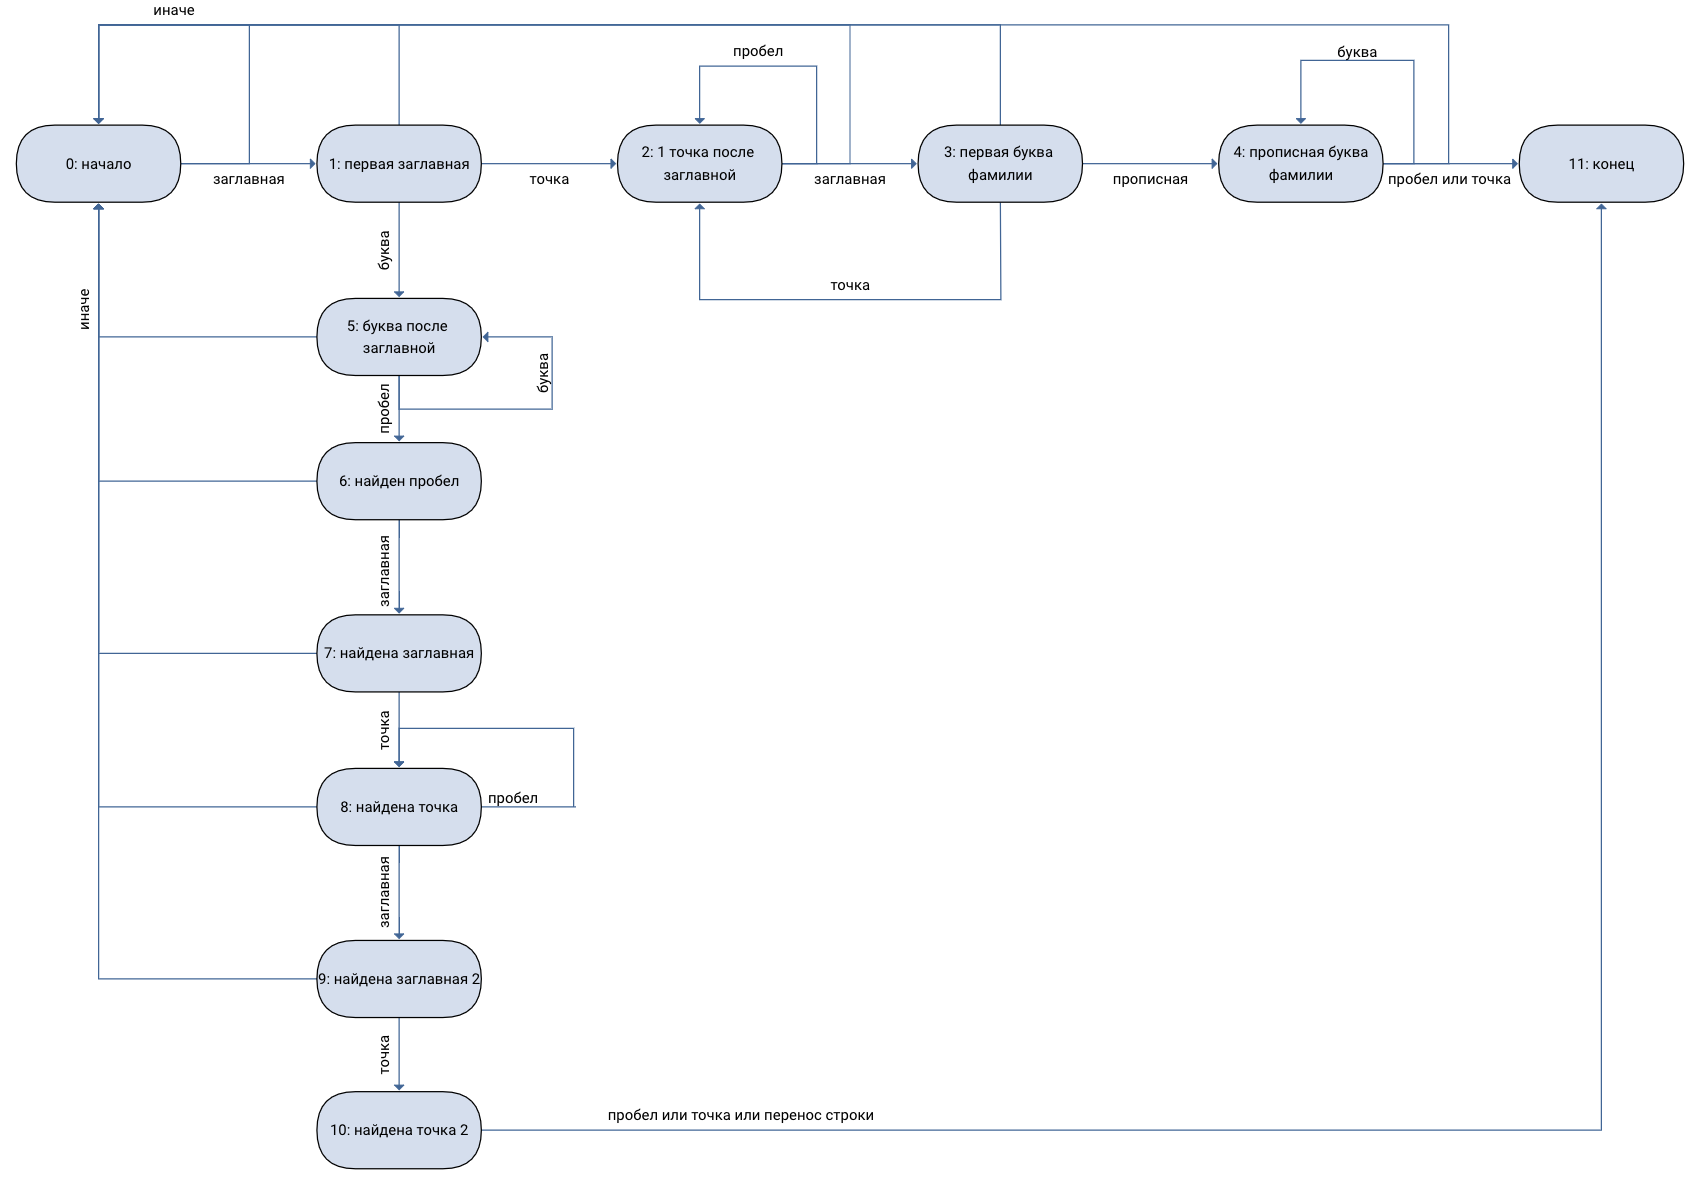
\includegraphics[scale=0.9]{graph.png}} 
	\caption{Конечный автомат}
	\label{ris:example}
\end{figure}

\section{Вывод}
В данном разделе был рассмотрен конечный автомат, на котором основан алгоритм и требования к работе программы.

\chapter{Технологическая часть}
\section{Выбор ЯП}
Я выбрал в качестве языка программирования Python, потому как данный язык имеет поддержку регулярных выражений и удобен для реализации конечного автомата.

\section{Листинг кода алгоритмов}
В данном разделе будет представлены листинги кода с помощью регулярных выражений (\ref{RegExp}), с помощью конечного автомата(\ref{Avt})
\begin{lstlisting}[label=RegExp,caption = Использование регулярных выражений]

    print("Регулярные выражения:")
    with open("data_1.txt", "r") as f:
        s = f.read()

    sm = 0
    while True:
        result = re.search(r'(([А-Я]\.\s?[А-Я]\.\s?[А-Я][а-я]{1,20})|([А-Я][а-я]{1,20}\s[А-Я]\.\s?[А-Я]\.))', s)

        if result is None:
            break
        print("Символы с %d до %d: "%(result.start()+1+sm, result.end()+1+sm) + s[result.start():result.end()])
        s = s[result.end():]
        sm += result.end()

\end{lstlisting}

\begin{lstlisting}[label=Avt,caption=Использование конечного автомата]

def get_symb_type(char):
    if len(char) == 0:
        return -1
    if char == '.':
        return 'dot'
    elif char == ' ':
        return 'space'
    elif ord('А') <= ord(char) <= ord('Я') or char == 'Ё':
        return 'capital'
    elif ord('а') <= ord(char) <= ord('я') or char == 'ё':
        return 'char'
    elif char == '\n':
        return 'n'
    else:
        return 'other'


def main():
    print("Конечный автомат:")
    file = open("data_1.txt", 'r')
    char = 1
    cnt = 0
    pos = 'begin'
    while char:
        char = file.read(1)
        cnt += 1

        type = get_symb_type(char)

        if pos == 'begin':
            if type == 'capital':
                pos = 'first_capital'
                first_symb = cnt

        elif pos == 'first_capital':
            if type == 'dot':
                pos = '1_dot_after_capital'
            elif type == 'char':
                pos = '2_char_after_capital'
            else:
                pos = 'begin'

        elif pos == '1_dot_after_capital':
            if type == 'space':
                continue
            elif type == 'capital':
                pos = '1_surname_capital'
            else:
                pos = 'begin'

        elif pos == '1_surname_capital':
            if type == 'char':
                pos = '1_char_after_surname_capital'
            elif type == 'dot':
                pos = '1_dot_after_capital'
            else:
                pos = 'begin'

        elif pos == '1_char_after_surname_capital':
            if type == 'char':
                continue
            else:
                pos = 'end'
                last_symb = cnt

        # '2_char_after_capital': 5,
        elif pos == '2_char_after_capital':
            if type == 'space':
                pos = '2_space_found'
            elif type == 'char':
                continue
            else:
                pos = 'begin'

        # '2_space_found': 6,
        elif pos == '2_space_found':
            if type == 'capital':
                pos = '2_capiatl_found_1'
            else:
                pos = 'begin'

        # '2_capiatl_found_1': 6,
        elif pos == '2_capiatl_found_1':
            if type == 'dot':
                pos = '2_dot_found_1'
            else:
                pos = 'begin'

        # '2_dot_found_1': 8,
        elif pos == '2_dot_found_1':
            if type == 'space':
                continue
            elif type == 'capital':
                pos = '2_capiatl_found_2'
            else:
                pos = 'begin'

        # '2_capiatl_found_2': 9,
        elif pos == '2_capiatl_found_2':
            if type == 'dot':
                pos = '2_dot_found_2'
            else:
                pos = 'begin'

        # '2_dot_found_2': 10,
        elif pos == '2_dot_found_2':
            pos = 'end'
            last_symb = cnt

        # 'end': 11
        elif pos == 'end':
            print("символы с", first_symb, "по", last_symb,": ", end='')

            with open("data_1.txt", "r") as f:
                print(f.read()[first_symb - 1:last_symb -1])

            pos = 'begin'

    file.close()

\end{lstlisting}


\section{Вывод}
В данном разделе была рассмотрена структура ПО и листинги кода программы.


\chapter*{Заключение}
\addcontentsline{toc}{chapter}{Заключение}
В ходе лабораторной работы были изучены возможности регулярных выражений. Были реализованы алгоритмы поиска ФИО в тексте при помощи регулярных выражений и конечного автомата.


\addcontentsline{toc}{chapter}{Список литературы}
\begin{thebibliography}{3}
	\bibitem{Fridl}
	Фридл, Дж. Регулярные выражения = Mastering Regular Expressions. — СПб.: «Питер», 2001. — 352 с. — (Библиотека программиста). 	\bibitem{Smith}
	Смит, Билл. Методы и алгоритмы вычислений на строках (regexp) = Computing Patterns in Strings. — М.: «Вильямс», 2006. — 496 с.
	\bibitem{Fort}
	Форта, Бен. Освой самостоятельно регулярные выражения. 10 минут на урок = Sams Teach Yourself Regular Expressions in 10 Minutes. — М.: «Вильямс», 2005. — 184 с.
\end{thebibliography}

\end{document}